
\documentclass[12pt]{article}
\usepackage{lmodern}
\usepackage[T1]{fontenc}
\usepackage[portuges]{babel}
\usepackage[utf8]{inputenc}
\usepackage{a4}
\usepackage{textgreek}
\usepackage{epstopdf}
\usepackage{graphicx}
\usepackage{fancyvrb}
\usepackage{amsmath}
\usepackage{float}
\usepackage{listings}
%\renewcommand{\baselinestretch}{1.5}


\begin{document}

\begin{titlepage}

\newcommand{\HRule}{\rule{\linewidth}{0.5mm}} % Defines a new command for the horizontal lines, change thickness here

\center % Center everything on the page
    
%----------------------------------------------------------------------------------------
%	HEADING SECTIONS
%----------------------------------------------------------------------------------------

\textsc{\LARGE Universidade do Minho}\\[1.5cm] 
\textsc{\Large Mestrado Integrado em Engenharia Informática}\\[0.5cm] 
\textsc{\large Computação Gráfica}\\[0.5cm]

%----------------------------------------------------------------------------------------
%	TITLE SECTION
%----------------------------------------------------------------------------------------

\HRule \\[0.4cm]
{ \huge \bfseries Transformações Geométricas}\\[0.4cm] 
\HRule \\[1.5cm]
    
%----------------------------------------------------------------------------------------
%	AUTHOR SECTION
%----------------------------------------------------------------------------------------

\begin{minipage}{0.4\textwidth}
\begin{flushleft} \large
\emph{Grupo:}\\
Etienne Costa A76089 \\
Joana Cruz A76270 \\
Rafael Alves A72629 \\
Maurício Salgado A71407 \\
\end{flushleft}
\end{minipage}
~
\begin{minipage}{0.4\textwidth}
\begin{flushright} \large
\emph{Docente:} \\
António Ramires\\
\end{flushright}
\end{minipage}\\[2cm]

%----------------------------------------------------------------------------------------
%	DATE SECTION
%----------------------------------------------------------------------------------------

{\large \today}\\[2cm]

%----------------------------------------------------------------------------------------
%	LOGO SECTION
%----------------------------------------------------------------------------------------


\includegraphics[scale=0.3]{uminho}\\
    
%----------------------------------------------------------------------------------------

\vfill % Fill the rest of the page with whitespace

\end{titlepage}
\tableofcontents
\newpage
\section{Introdução}
O relatório apresentado diz respeito à segunda fase  do projeto proposto no âmbito da unidade curricular de
Computação Gráfica. O trabalho consiste na criação de um cenário através do processamento de ficheiros XML e aplicação de várias
transformações geométricas em OpenGL tal como translações, rotações e escalas.
Numa primeira fase é explicado o modo como desenvolvemos as estruturas de dados que suportam o programa, posteriormente será descrito
o processo de leitura e tratamento dos dados contidos no ficheiro XML e e por último a utilização de VBO's e o modo como
cada elemento é renderizado na função renderscene. No final do relatório encontram-se alguns exemplos de execução.
\newpage
\section{Engine}
O programa Engine está dividido em duas fases: leitura, extração de dados de ficheiros
XML para armazenamento em estruturas apropriadas e o desenho das cenas com o auxílio de eventuais primitivas gráficas.
Na primeira fase, o programa lê os ficheiros XML, extraindo as suas informações,
nomeadamente o que diz respeito aos grupos - os modelos que contém e as outras operações em OpenGL a efetuar
(translações, rotações e escalas), assim como a sua cor.
Na segunda fase, o programa encarrega-se de desenhar a cena descrita no ficheiro XML
através de um ciclo de rendering.
Com os novos ficheiros de configuração XML de entrada pedidos nesta fase, foi necessário reestruturar o engine e o parser, assim 
como desenvolver classes para armazenamento da informação pretendida.
Como já foi referido no relatório anterior, o programa possui ainda funcionalidades relativas ao movimento da cena:
\begin{itemize}
\item deslocação de um modelo com as teclas - \textit{a, d} para translações no eixo dos xx; \textit{w, s} para translações no eixo dos yy; \textit{4, 5} para translações no eixo dos zz 
\item rotação de um modelo com as setas do teclado através da camera
\item rotação no eixo vertical de um modelo com teclas \textit{q, e} com recurso à função glRotatef
\item definição de opções Fill, Line ou Point em OpenGL relativas ao desenho dos modelos com as teclas \textit{f,l,p}
\item zoom in e zoom out com teclas \textit{x, z}
\end{itemize}
\newpage
\section{Estruturas de dados}
Devido à necessidade de guardar diferentes tipos de informações, lidas a partir
do ficheiro XML e posteriormente usadas para desenhar o cenário sistema
solar, definimos as seguintes estruturas de dados.
\subsection{Vertex}
Esta classe representa um ponto num referencial a três dimensões, com as
coordenadas x, y e z, o que se torna bastante útil para a representação dos
vértices utilizados posteriormente para o desenho dos triângulos que elaboram as figuras primitivas.
\begin{lstlisting}
class Vertex{
public:
	float x;
	float y;
	float z;
	Vertex();
	Vertex(float xx, float yy, float zz);
	~Vertex();
};
\end{lstlisting}
\subsection{Model}
Esta classe armazena todos os pontos para a criação das figuras primitivas (plane, box,
cone, sphere) que estão presentes e descritos no ficheiro.
\begin{lstlisting}
class Model{
public:
	string fileName;
	vector<Vertex> vertexes;
	Model();
	Model(string path);
	~Model();
};
\end{lstlisting}
\subsection{Group}
Esta é a classe que guarda os dados retirados de um grupo do ficheiro XML.
Nesta estrutura é possível armazenar todas as informações que estão associadas a um determinado grupo, as respetivas 
transformações geométricas se existirem, os modelos associados a esse grupo, assim como os grupos filhos contidos. Decidimos também
guardar a cor no grupo. Como as seguintes transformações geométricas - translações e escalas - acabam por ser um ponto com três coordenadas do tipo float,
decidimos utilizar a classe acima definida Vertex. O mesmo se passa com as rotações,
apenas com a particularidade que também existe um ângulo de rotação, daí esse ser armazenado também.
\begin{lstlisting}
class Group{
public:
	Vertex rotation;
	float rotationAngle;
	Vertex translation;
	Vertex scale;
	Vertex color;
	vector<Model> models;
	vector<Group> subGroups;
	Group(void);
	Group(Vertex rotation, float rotAngle,
	Vertex translation, Vertex scale, Vertex color, 
	vector<Model> models, vector<Group> subGroups);
	~Group();
};
\end{lstlisting}
\newpage
\section{Processamento de um ficheiro XML}
O processamento de um cenário em formato XML pode ser visto como duas fases
distintas:
\begin{itemize}
\item Leitura e Processamento do cenário – Consiste na abertura do ficheiro que contém o
cenário que em modo de leitura e extração da respetiva hierarquia em XML. Nesta
fase são também retiradas as componentes que caraterizam uma
transformação geométrica (translação, escala ou rotação), a cor do grupo ou desenho de uma
primitiva.
\item Armazenamento nas estruturas de dados – De modo a se conseguir redesenhar
um modelo quantas vezes for necessário, em estruturas acima referidas.
Na nossa função main do programa apenas lemos o ficheiro uma vez e armazenamos nas estruturas apropriadas.
\end{itemize}
\subsection{Parser}
Esta é a classe que efetua o processo acima descrito. Agora fazemos uma pequena descrição sobre os métodos utilizados.
\begin{itemize}
\item ParseXMLFile - sendo a cena sempre um conjunto de grupos, esta função verifica se o documento XML apresenta um formato
correto e após isso vai começar a efetuar o parsing de cada grupo
\item ParseGroup - percorre um nodo do tipo grupo do XML e extrai a informação correspondente. Se o grupo em questão
contiver outros grupos dentro de si, essa informação também será processada. Esta função faz o controlo de possíveis ficheiros
de configuração XML errados, caso exista mais que uma transformação do mesmo tipo num grupo, apenas processa a primeira.
Caso a informação a ler seja uma transformação geométrica a função parseAttributes é invocada
\item ParseModel - processa a informação correspondente ao ficheiro da figura primitiva
\item ParseAttributes - processa a informação sempre que é encontrada uma transformação (traslate, rotate ou scale) criando
um vértice e adicionando-o ao grupo que está a ser gerado pelo
parseGroup.
\end{itemize}
\newpage
\section{Utilização de VBO's}
Vertex Buffer Objects podem ser vistos como uma estrutura abstrata de dados que permite melhorar
consideravelmente a performance geral do OpenGl.
A vantagem de usar um VBO é a seguinte:
\begin{itemize}
\item Sem a utilização de VBOs, utilizando o modo de desenho imediato do OpenGL,
os vértices são definidos em memória RAM e copiados um a um, para a placa
gráfica, conforme a ordem com que devem ser processados. Este processo é
repetido sempre que os queremos desenhar.
\item Com a utilização VBOs, todos os vértices são definidos e copiados para um buffer,
que é passado numa fase inicial, e uma única vez, para a memória da placa
gráfica, antes de qualquer pedido para os processar e desenhar.
Deste modo, o processamento dos triângulos a desenhar torna-se muito mais
eficiente.
\end{itemize} 
Apesar de apenas ser pedido na próxima fase, decidimos já implementar o desenho das primitivas recorrendo ao uso de VBO's, dado a 
estas questões de performance. Para isso no nosso motor, após a leitura e processamento do ficheiro,
começamos por gerar quantos buffers quanto o número de grupos que temos com recurso à função \textbf{glGenBuffers}.
De seguida, para preencher cada um dos VBOs com as coordenadas dos vértices, relativos a um determinado grupo criámos um método \textbf{fillBuffers}.
Neste método, é feito um ciclo para iterar cada um dos grupos, e preencher cada um dos índices do array de VBOs com as coordenadas
dos vértices dos respetivos modelos do grupo. Tendo preenchido o array com as coordenadas, é ativada a posição do array de VBOs
sobre o qual se vão inserir os dados, com recurso à função \textbf{glBindBuffer}. O referido índice
é preenchido com os elementos do array de coordenadas determinado, usando para isso
a função \textbf{glbufferData}.
Como no preenchimento dos VBOs deve também ser tida em consideração a ordem
pela qual os grupos são processados, caso o nó recebido como argumento tenha filhos,
a função é chamada recursivamente para o respetivo Grupo filho. Só depois desta
verificação, é que caso existam irmãos no nodo, a função é iterada recursivamente para
o Grupo irmão.\newline
\newpage
\section{Ciclo de rendering}
Primeiramente decidimos explicar os conceitos das funções 
\textbf{glPushMatrix()} e \textbf{glPopMatrix()}, que se tornaram bastante importantes para o correto desenho do cenário.
Para conseguir preservar um estado da matriz de visualização de um
determinado modelo, é utilizada a função \textbf{glPushMatrix()} da biblioteca glut, que irá
guardar a matriz atual numa stack.
Quando for pretendido recuperar a última matriz guardada na referida stack, basta para isso utilizar a
a função \textbf{glPopMatrix()}.\newline
Tendo em conta os conceitos mencionados será descrito o processo utilizado para a
execução do ciclo de rendering.
Decidimos implementar uma função drawScene que será invocada no renderScene 
e irá percorrer a estrutura de dados final - uma lista de objectos
do tipo Group.
\begin{enumerate}
\item Antes de realizar qualquer alteração à matriz de visualização do modelo é
efetuado um \textbf{glPushMatrix()} de modo a guardar o estado da matriz atual
\item Após isso, são realizadas as transformações correspondentes, por esta ordem
uma rotação, uma translação e uma escala que vão ser
aplicadas à matriz atual, utilizando as funções do glut \textbf{glRotatef}, \textbf{glTranslatef} e \textbf{glScalef} respetivamente. 
Define-se também a cor a aplicar aquele grupo
\item Realizadas as transformações, ativa-se o buffer correspondente e 
vão ser desenhados todos os vértices dos modelos do grupo, com recurso às funções
\textbf{glVertexPointer} e \textbf{glDrawArrays}
\item Caso o nodo atual tenha
descendência, a função drawScene é chamada recursivamente para o filho,
sem que o \textbf{glPopMatriz()} seja efetuado, para que não se percam as
transformações já realizadas
\item Caso o grupo atual não tenha nenhum grupo filho, é finalmente efetuado o \textbf{glPopMatrix()},
uma vez que vamos querer voltar ao estado da matriz de visualização do modelo
anterior, sem as alterações que foram efetuadas pela atual iteração da função
drawScene. Este processo é efetuado porque as transformações dos grupos
seguintes já não serão sobrepostas às transformações atuais
\end{enumerate}
\newpage
\section{Exemplos de Execução}
\subsection{Figuras primitivas}
Exemplo de um cenário básico contendo algumas transformações geométricas e diferentes primitivas gráficas.
\begin{figure}[H]
\centering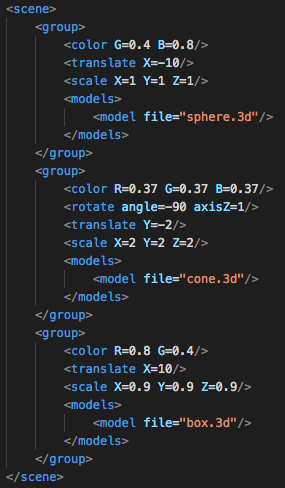
\includegraphics[scale=0.80]{xmlPrimitives} 
\caption{\label{fig:controller}Ficheiro XML para um exemplo com algumas primitivas e transformações}
\end{figure}
\begin{figure}[H]
\centering
\includegraphics[scale=0.35]{primitives} 
\caption{\label{fig:controller}Cenário com as primitivas gráficas}
\end{figure}
\subsection{Figuras primitivas com diferentes escalas}
\begin{figure}[H]
\centering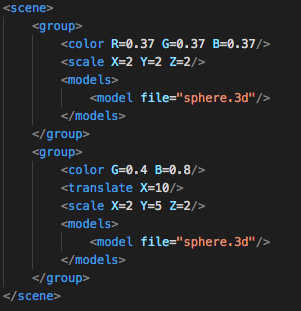
\includegraphics[scale=0.80]{xmlScales} 
\caption{\label{fig:controller}Ficheiro XML para demonstrar a mesma primitiva com diferentes escalas}
\end{figure}
\begin{figure}[H]
\centering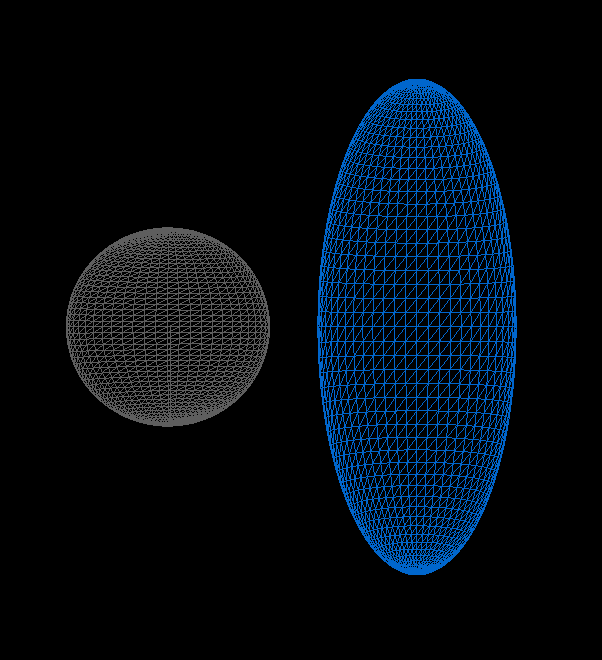
\includegraphics[scale=0.50]{scales} 
\caption{\label{fig:controller}Cenário com as primitivas gráficas com diferentes escalas}
\end{figure}
\subsection{Sistema solar estático}
Para o nosso cenário do sistema solar estático desenvolvemos dois ficheiros de configuração XML.
Em ambos os ficheiros, para cada planeta do Sistema Solar criamos um grupo irmão,
mas para as luas de um planeta usamos como base as tranformações já efetuadas no planeta e aplicamos as
novas transformações necessárias. A primitiva gráfica usada para o desenho do Sol, de cada planeta, das luas e 
do anel de Saturno é sempre a esfera, com diferentes escalas aplicadas.
Neste primeiro cenário, são apenas aplicadas translações e escalas, e apenas uma rotação para o anel de Saturno.
Neste os planetas ficam todos alinhados no eixo dos xx com excepção das luas.  
\begin{figure}[H]
\centering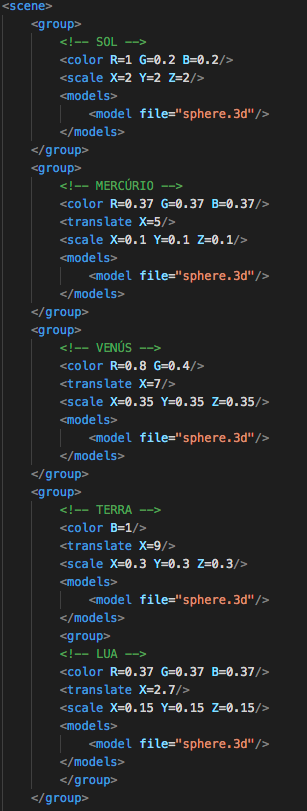
\includegraphics[scale=0.80]{xmlSolar} 
\caption{\label{fig:controller}Excerto do exemplo de um ficheiro XML de um Sistema Solar estático}
\end{figure}
\begin{figure}[H]
\centering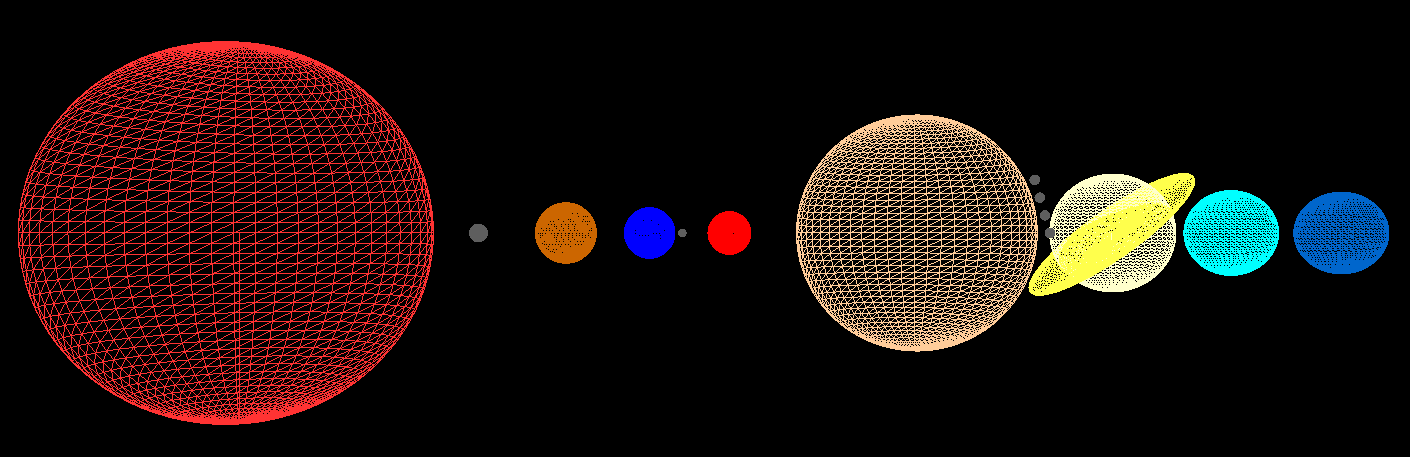
\includegraphics[scale=0.30]{solar} 
\caption{\label{fig:controller}Cenário de um Sistema Solar estático}
\end{figure}
\newpage
Já neste ficheiro decidimos aplicar rotações no eixo dos yy, para conseguirmos modificar a direção dos eixos dos xx e zz, aplicando
as devidas translações de seguida.
\begin{figure}[H]
\centering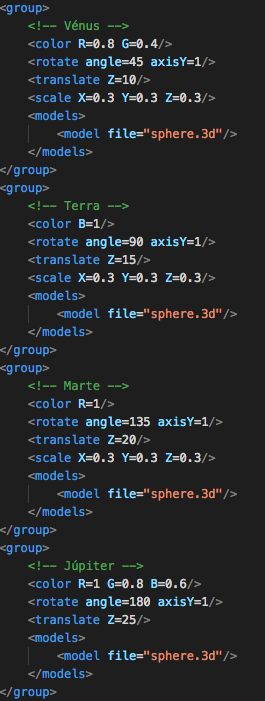
\includegraphics[scale=0.70]{xmlSolar1} 
\caption{\label{fig:controller}Excerto do exemplo de um ficheiro XML de um Sistema Solar estático}
\end{figure}
\begin{figure}[H]
\centering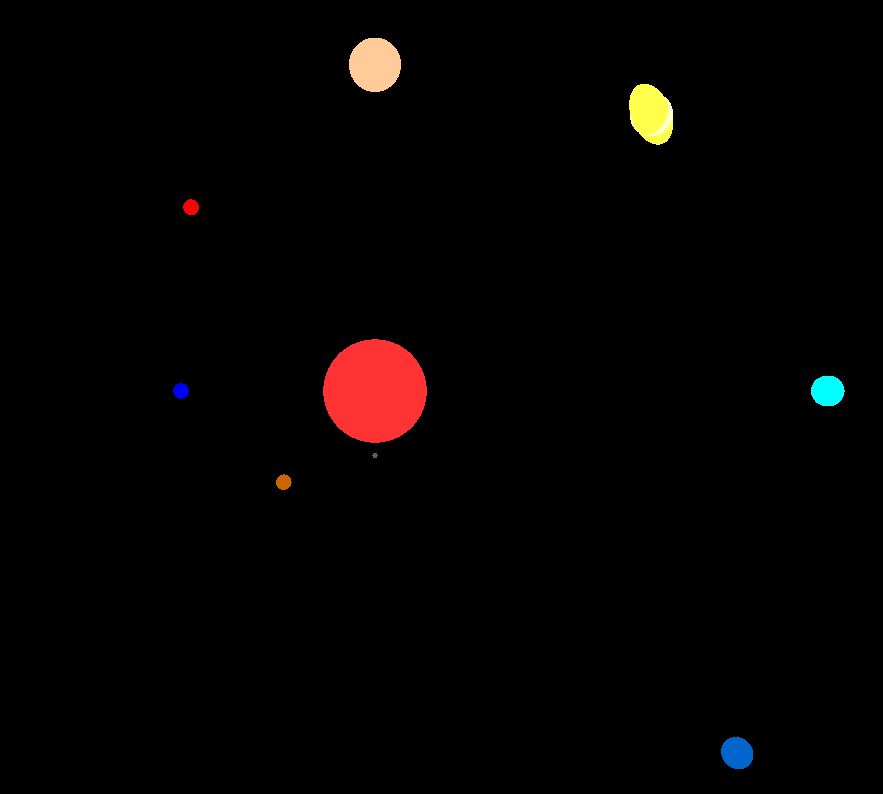
\includegraphics[scale=0.40]{solar1} 
\caption{\label{fig:controller}Cenário de um Sistema Solar estático}
\end{figure}
\newpage
\section{Conclusão}
Nesta segunda fase inicialmente encontramos algumas dificuldades na interpretação do ficheiro XML, assim como 
a melhor abordagem para a sequência de transformações - se primeiro aplicar uma rotação e só após uma translação ou o contrário - 
que após uma análise detalhada foram ultrapassadas. Desenvolvemos
o nosso conhecimento de OpenGL, pois com a introdução das transformações, evoluímos bastante
sobre como manipular as matrizes de forma a que o desenho das primitivas gráficas fosse nas posições pretendidas. Quanto à 
aplicação Engine, várias alterações foram feitas, devido ao aumento da dimensão do projeto, decidimos estruturar em classes e segmentar o código.
Cumprimos todos os requisitos propostos, apenas ficou por otimizar o nosso processamento de leitura de ficheiros de configuração XML caso encontre 
um ficheiro XML inválido com múltiplas transformações do mesmo tipo. Além do trabalho futuro já proposto na próxima fase,
iremos desenvolver uma figura primitiva Torus para o desenho do anel de Saturno.
\end{document}